\part{Ondas}


\begin{myalertblock}{Ondas}
En física, se conoce como onda a la propagación de energía (y no de masa) en el espacio debido a la perturbación de alguna de sus propiedades físicas, como son la densidad, presión, campo eléctrico o campo magnético. Este fenómeno, , sumamente común en el universo, puede darse en un espacio vacío o en uno que contenga materia (aire, agua, tierra, etc.).

\vspace{2mm} De acuerdo al origen de las ondas o de la naturaleza del medio a través del cual se propagan, dependerán los efectos de su aparición y sus características. Así, podemos hablar de ondas de luz, de sonido, etc., cada una con propiedades físicas y frecuencias diferentes, dependiendo, entre otras cosas, del medio en el que se propagan y de cuánta energía transportan.
Algunas ondas, como las sonoras, no pueden transportarse en el vacío, requieren de un medio físico. Otras, como las ondas electromagnéticas, pueden hacerlo perfecta y velozmente.

\vspace{2mm} Podemos clasificar las ondas de acuerdo al medio en que se propagan como:

--- Ondas mecánicas. Precisan de un medio elástico (líquido, gaseoso o sólido) y de condiciones determinadas de temperatura y presión, para propagarse efectivamente. Por ejemplo: las ondas sonoras que se propagan por el aire o por el agua.

--- Ondas electromagnéticas. No requieren de un medio de propagación,  se pueden propagar en el vacío. Por ejemplo: la luz.

--- Ondas gravitatoria. Perturbaciones del espacio-tiempo producida por un cuerpo masivo acelerado. La existencia de ese tipo de onda, que consiste en la propagación de una perturbación gravitatoria en el espacio-tiempo y que se transmite a la velocidad de la luz, fue predicha por Einstein en su teoría de la relatividad general.

\begin{figure}[H]
		\centering
		
\includegraphics[width=1\textwidth]{imagenes/imagenes19/T19IM01.png}
	\end{figure}

Según el movimiento del medio, las ondas son:

--- Ondas longitudinales. Las partículas del medio se mueven en la misma dirección en que se propaga la onda.

--- Ondas transversales. Las partículas vibran perpendicularmente a la dirección de propagación de la onda.


\vspace{2mm} Se puede describir todas las ondas mediante tres características:

--- amplitud que corresponde a la altura de las oscilaciones;

--- longitud de onda que mide la distancia entre dos oscilaciones:

--- frecuencia que refleja el número de oscilaciones por segundo (expresado en hercios e inversamente proporcional a la longitud de onda).
\end{myalertblock}

\chapter{Movimiento armónico simple}

\vspace{-5mm} %************************************
\begin{miparrafo}
\small{El movimiento armónico simple (M.A.S.), también denominado movimiento vibratorio armónico simple (m.v.a.s.), es un movimiento periódico de vaivén en el que un cuerpo oscila de un lado a otro de su posición de equilibrio y en intervalos de tiempo iguales. Algunos ejemplos de este movimiento son el movimiento de un péndulo simple o el movimiento de una partícula oscilante sujeta a un resorte que se ha comprimido.}

\begin{multicols}{2}
\small{En el caso de que la trayectoria sea rectilínea, la partícula que realiza un m.a.s. oscila alejándose y acercándose de un punto, situado en el centro de su trayectoria, de tal manera que su posición en función del tiempo con respecto a ese punto es una sinusoide. En este movimiento, la fuerza que actúa sobre la partícula es proporcional a su desplazamiento respecto a dicho punto y dirigida hacia este.	}
\begin{figure}[H]
		\centering
		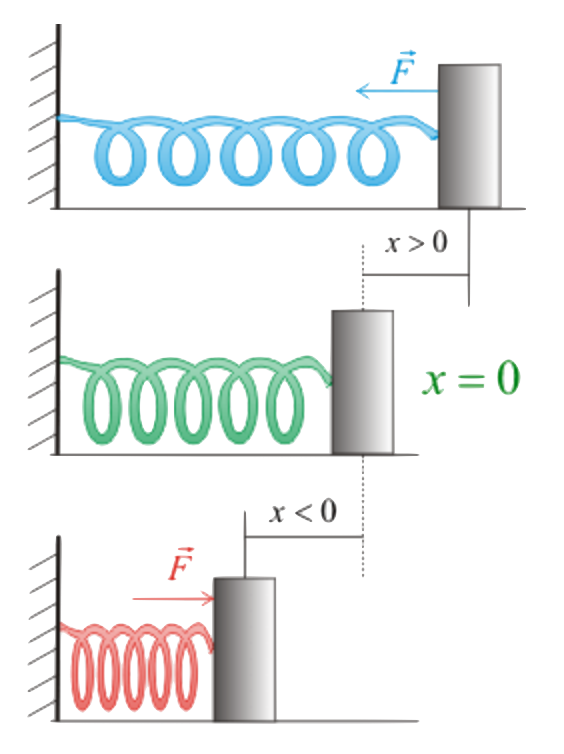
\includegraphics[width=.4\textwidth]{imagenes/imagenes19/T19IM02.png}
	\end{figure}
\end{multicols}
\end{miparrafo}

\section{Introducción}
Un fenómeno variable con el tiempo es un \emph{fenómeno periódico} de periodo $T$ cuando todas las variables que caracterizan al movimiento (posición, velocidad, aceleración, $cdost$) toman el mismo valor en los instantes $t$ y $t+T$, $\forall t$.

El \emph{movimiento oscilatorio} es el de una partícula que se mueve periódicamente respecto a una posición llamada posición de equilibrio.

Sea $\psi$ una magnitud cualquiera variable con el tiempo, $\psi=F(t)$, $\psi$ es periódica si $F(t+T)=F(t)$.

Se define la \emph{frecuencia} como el número de periodos que tienen lugar en la unidad de tiempo, $\nu=\dfrac 1 T$. Su unidad en el $SI$ recibe el nombre de \emph{hertz}\footnote{La unidad de frecuencia lleva el nombre del físico alemán Heinrich Rudolf Hertz (1857-1894)}, $\mathrm{Hz}$, que equivale a 1 ciclo $\mathrm{s}^{-1}$.

La mayor parte de los fenómenos periódicos llegan a alcanzar el reposo, se llaman \emph{movimientos amortiguados}.

El movimiento periódico más importante de la física matemática es el MAS, \emph{movimiento armónico simple.}

\section[Cinemática de movimiento armónico simple]{Cinemática de movimiento armónico simple\sectionmark{Cinemática del MAS}}
\sectionmark{Cinemática del MAS}

Decimos que una partícula que se mueve a lo largo de un eje describe un MAS cuando la ecuación matemática que representa su posición viene dada por la siguiente expresión:

\begin{equation}
\label{MAS-definicion}
\subrayado{ \ \boldsymbol{x\ =\ A\ cos (\omega t+\alpha) } \ }	
\end{equation}

Donde:$\quad \omega t + \alpha\ $ es la \textbf{fase}; $\quad \alpha \ $ es la \textbf{fase inicial} ($t=0$); $\quad A \ $ es la \textbf{amplitud} del MAS y $\quad \omega \ $ la \textbf{velocidad angular, pulsación o frecuencia angular}.

La posición $x$ recibe el nombre de \textbf{elongación}. La amplitud $A$ es el valor máximo que puede tomar la elongación en un MAS \scriptsize{ \{ $\cos \omega t+\alpha) \in [-1,1]$ \} }\normalsize{.}

Como el MAS es un movimiento periódico,

$A\cos(\omega t + \alpha)=A\cos (\omega (t+T)+\alpha) \ \to \ 2\pi +\cancel{\omega t} + \cancel{\alpha}= \omega (\cancel{t}+T) + \cancel{\alpha} $

\begin{equation}
\label{MAS-T}
\subrayado{ \ \boxed{\ \boldsymbol{T=\dfrac {2\pi}{\omega}} \quad \leftrightarrow \quad \omega=\dfrac{2\pi}{T} \ } \ }
\end{equation}

Vamos a determinar la velocidad del MAS:

$\displaystyle v=\dv{x}{t}=-A\omega \sin (\omega t + \alpha)= A \omega \cos \left( \omega t + \alpha + \dfrac \pi 2 \right)$

--- La diferencia de fase entre velocidad y elongación en un MAS es de $\dfrac \pi 2$.

Vamos a por la aceleración:

$\displaystyle a=\dv[2]{x}{t}=\dv{v}{t}=-A \omega^2 \cos(\omega t + \alpha)=A\omega^2 \cos(\omega t + \alpha + \pi)$

--- La diferencia de fase entre aceleración y elongación en un MAS es de $\pi$ radianes.


También podemos considerar el MAS como aquel movimiento que describe la proyección de una partícula sobre un eje cuando la partícula se mueve sobre un circulo con $\omega$ constante.

\begin{multicols}{2}
El vector velocidad esta asociado al vector  $\overrightarrow{OP}'$ de dimensión $A\omega$ y que se mueve con $\omega=cte$ y con $\frac \pi 2$ de diferencia de fase con la elongación.

La aceleración es la proyección de  $\overrightarrow{OP}''$, de longitud $A\omega^2$ y con $\pi$ radianes de diferencia de fase respecto a la elongación.

\begin{figure}[H]
		\centering
		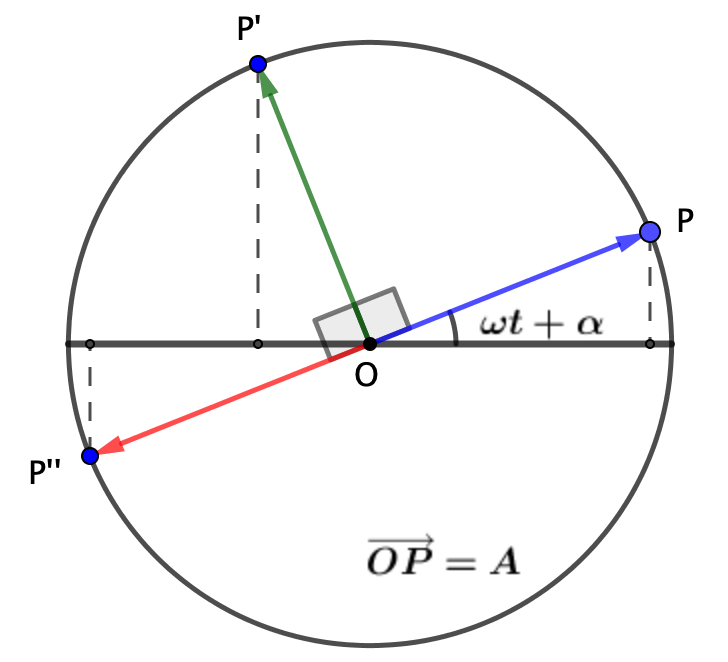
\includegraphics[width=.4\textwidth]{imagenes/imagenes19/T19IM03.png}
	\end{figure}
\end{multicols}

\begin{figure}[H]
		\centering
		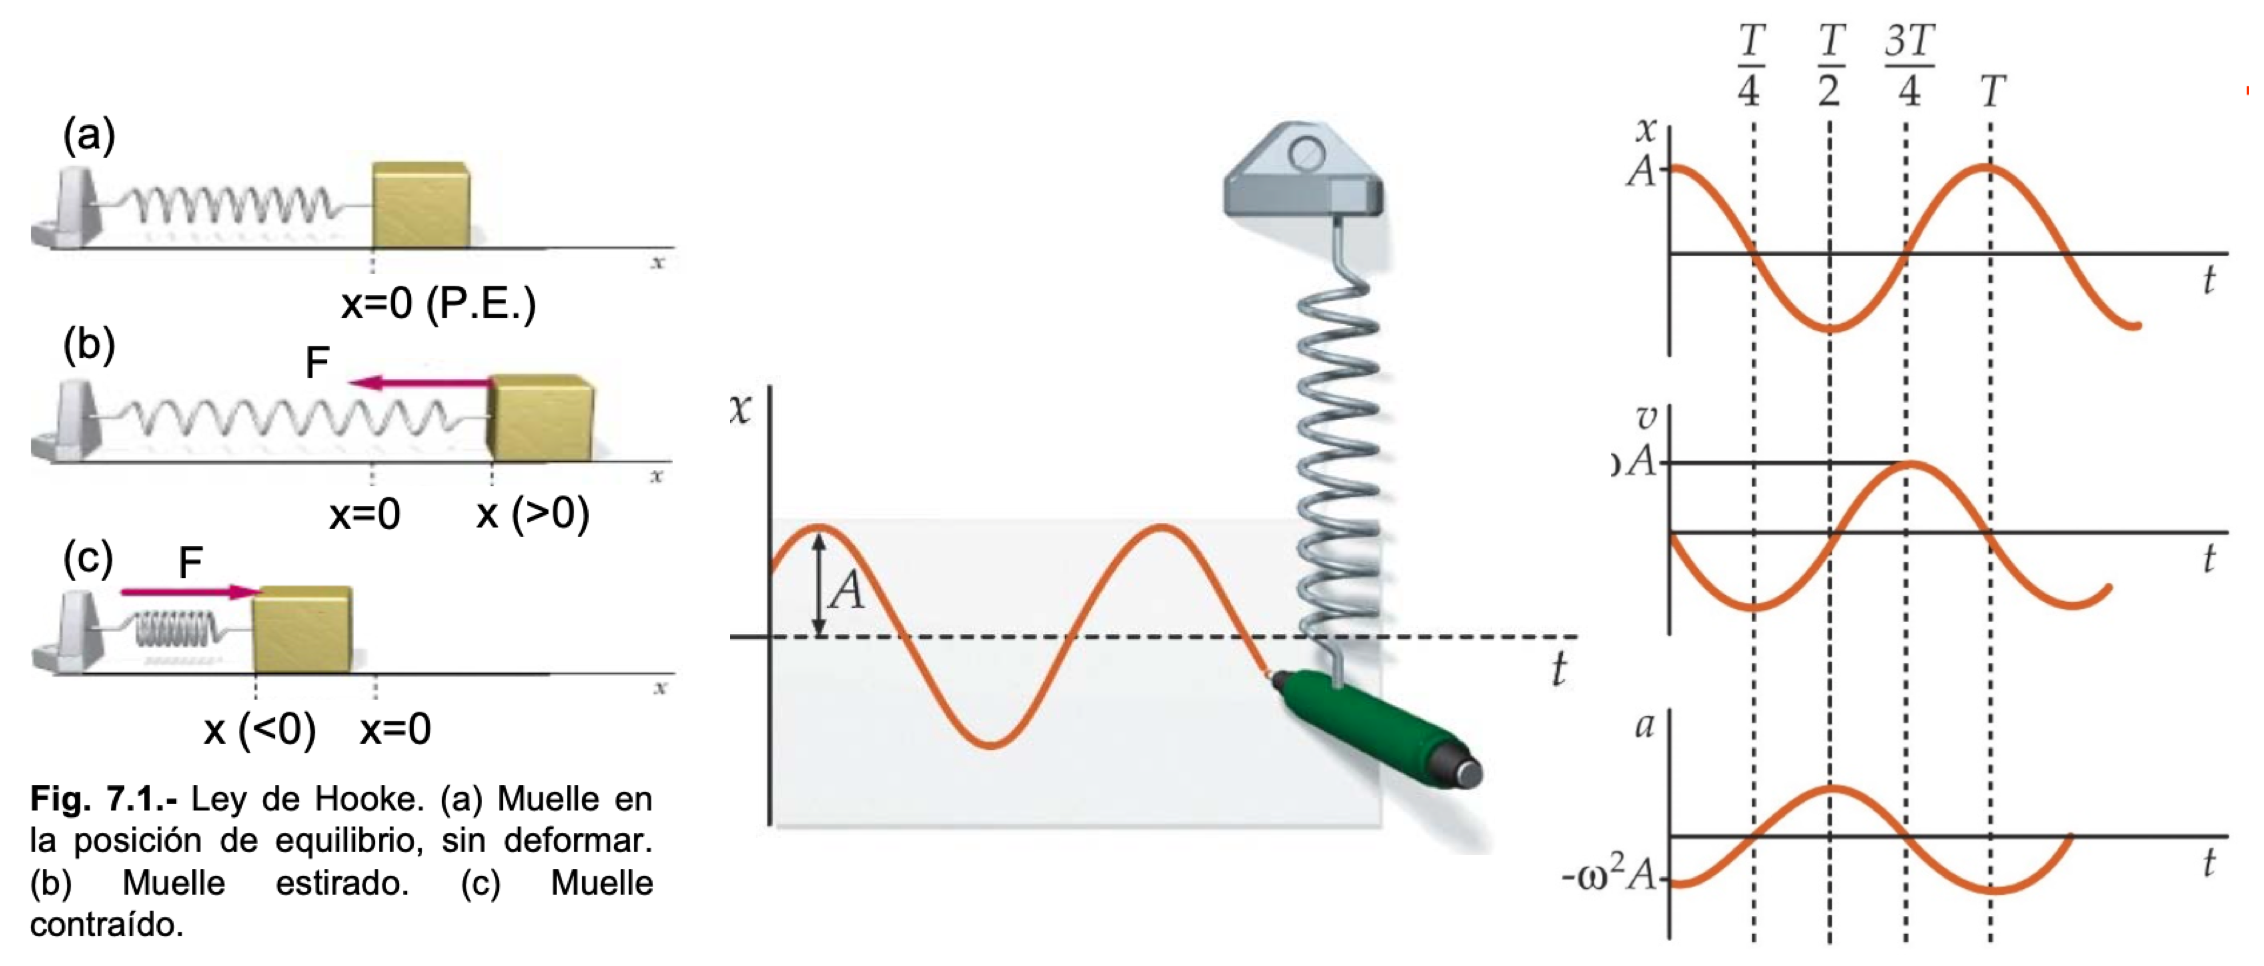
\includegraphics[width=1\textwidth]{imagenes/imagenes19/T19IM04.png}
	\end{figure}
	
\section{Fuerza y energía en el MAS}

Segunda ley de Newton. Suponemos que se conserva la masa y que el movimiento es unidimensional:

\begin{equation}
\label{MAS-F}
\subrayado{ \ \boxed{\ \boldsymbol{ \ F=\ \textcolor{gris}{ma} \ =-m\ \omega^2 \ x} \ } \ }	
\end{equation}

En el MAS, la fuerza es proporcional a la elongación, siendo el producto de la masa por el cuadrado de la velocidad angular la constante de proporcionalidad.

Comparando esta fuerza con la que sufre un muelle cuando se desplaza levemente de su posición original, Ley de Hooke $F=-kx$ ( subapartado - \ref{Hooke}), tenemos: 
$\ k=m\omega^2 \ $, con $k$ la constante elástica. Por otra parte, como $ \ \omega=\frac {2\pi}{T} \ $, tendremos que:

$$\subrayado{\ T=2\pi \ \sqrt{\dfrac{k}{m}} \ }; \quad \text{\small{Periodo oscilación muelle}\normalsize{.}}$$

Veamos cual es la energía cinética de una partícula en un MAS:

$\mathcal E_c=\dfrac 1 2 m v^2 = \frac 1 2 m A^2 \omega^2 \sin^2 (\omega t + \alpha) = \frac 1 2 m A^2 \omega^2 \left( 1 - \cos^2 (\omega t + \alpha) \right)$

Teniendo en cuenta la ecuaciónde definición del MAS, ec(\ref{MAS-definicion}), tenemos que

\begin{equation}
\subrayado{\ \mathcal E_c=\dfrac 1 2 m\omega^2 \left[ A^2-x^2 \right] = \dfrac 1 2 K \left[ A^2-x^2 \right] \ }; \quad \text{\small{en el caso de muelles}\normalsize{.}}
\end{equation}

Una consecuencia importante de la expresión de la $\mathcal E_c$ para el MAS es que, al ser siempre positiva ($x\leq A$), nos proporciona los \emph{\textbf{puntos de retorno}} cuando $\mathcal E_c=0 \to x=\pm A$

Al estar en un campo de fuerzas central (muelle), es conservativo y, por tanto, se conserva la energía mecánica. En un punto se anula la velocidad, se anula pues la energía cinética; un instante después se invierte el signo de la velocidad por exigencias del teorema de la conservación de la energía y la energía cinétita vuelve a aumentar hasta llegar a su valor máximo en $x=\pm A$.

\vspace{10mm} %************************************************
Campo conservativo, $\ \displaystyle F=-\pdv{\mathcal E_p}{x} \to \dd \mathcal E_p=-F\dd x=m\omega^2 x \dd x$

$\mathcal E_p=\dfrac 1 2 m \omega^2 x^2 + cte;\qquad  x=0 \ \to \ \mathcal E_p(0)=0=cte$, por lo que

\begin{equation}
	\subrayado{ \ \mathcal E_p \ = \ \dfrac 1 2 m \omega ^2  x^2 = \dfrac 1 2 K x^2 \ }; \quad \text{\small{en el caso de muelles}\normalsize{.}}
\end{equation}

\vspace{10mm} %************************************************
La energía mecánica, suma de cinética y potencial, para un MAS es:

\begin{equation}
\subrayado{\ \boldsymbol{E}= \ } \mathcal E_c+\mathcal E_p=\dfrac 1 2 m \omega^2 (A^2-x^2)+\dfrac 1 2 m \omega^2 x^2 = \subrayado{ \ \boldsymbol{\dfrac 1 2 m \omega^2 A^2=\dfrac 1 2 K A^2} \ }	
\end{equation}

\small{La última expresión válida para el caso de un muelle\normalsize{.}

Como cabía esperar, la energía mecánica se conserva, es constante.

\vspace{20mm} %************************************************
\begin{multicols}{2}
Energía potencial de un oscilador armónico (muelle):

La línea horizontal representa la energía total para la amplitud $A$.

La energía cinética es $\mathcal E_c=E-\mathcal E_p$.

Como la energía total es siempre mayor o igual a la energía potencial ($\mathcal E_c\geq 0$), el movimiento está restringido a: $ -A\leq x \leq A$	
\begin{figure}[H]
		\centering
		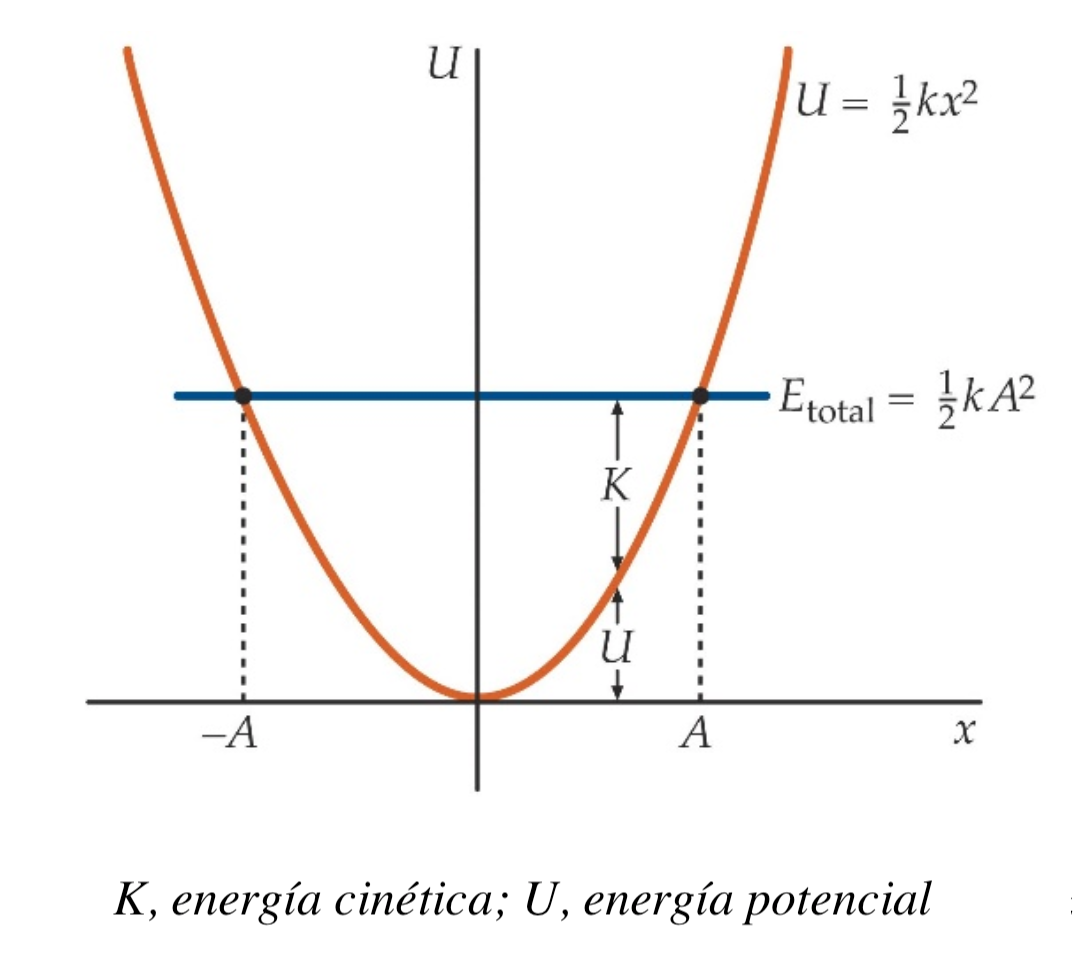
\includegraphics[width=.5\textwidth]{imagenes/imagenes19/T19IM05.png}
	\end{figure}
\end{multicols}

\section[Ecuaciones diferenciales de segundo orden con coeficientes constantes]{Ecuaciones diferenciales de segundo orden con coeficientes constantes\sectionmark{EDO segundo orden}}
\sectionmark{EDO segundo orden}

Al tipo de ecuaciones de movimiento siguiente se les llama \emph{ecuaciones diferenciales de segundo orden con coeficientes constantes}\footnote{Para ampliar información, consúltese el apéndice \ref{EDO}}:

\begin{table}[H]
\centering
\begin{tabular}{l}
	$\ (1) \quad \displaystyle a_2 \ \dv[2]{x}{t}+a_1\ \dv{x}{t}+a_0\ x=0$ \\ \\
	$\ (2) \quad \displaystyle a_2 \ \dv[2]{x}{t}+a_1\ \dv{x}{t}+a_0\ x=F(t)$
\end{tabular}
\end{table}

donde, $a_0,\ a_1,\ a_2=ctes$, $x$ es la variable independiente, $t$ la variable independiente.

A la ecuación $(1)$ se la llama \emph{ecuación homogénea} o incompleta y a la $(2)$ ecuación completa.

Vamos a ver tres teoremas.

\begin{teor}
Si $x=x_1(t)$ es una solución cualquiera de una 	ecuación diferencial de segundo orden con coeficientes constantes homogénea y $\mathcal C$ es una constante arbitraria, \textsf{entonces} la función $x=\mathcal C _1(t)$ también es solución.
\end{teor}
\begin{proof}\textcolor{white}{.}

$\displaystyle \mathcal C a_2 \dv[2]{x}{t}+\mathcal Ca_1 \dv{x}{t}+\mathcal C a_0=\mathcal C \cancelto{0}{ \left( a_2  \dv[2]{x}{t}+a_1 \dv{x}{t}+a_0 x \right) } = 0 $	
\end{proof}

\begin{teor}
	Si $x=x_1(t)$ y $x=x_2(t)$ son soluciones cualesquiera de una 	ecuación diferencial de segundo orden con coeficientes constantes homogénea, \textsf{entonces} la suma, $x=x_1(t)+x_2(t)$, también es solución.
\end{teor}
\begin{proof}
	$\displaystyle  \quad 
	a_2 \dv[2]{(x_1+x_2)}{t}+a_1 dv{(x_1+x_2)}{t}+a_0(x_1+x_2) = $
	
	$\displaystyle 
	\cancelto{0}{\left( a_2 \dv[2]{x_1}{t}+a_1\dv{x_1}{t}+a_0 x_1 \right)} +
		\cancelto{0}{\left( a_2 \dv[2]{x_2}{t}+a_1\dv{x_2}{t}+a_0 x_2 \right)} =0$
\end{proof}

\begin{coro}
	Si $x=x_1(t)$ y $x=x_2(t)$ son soluciones cualesquiera de una 	ecuación diferencial de segundo orden con coeficientes constantes homogénea, y $\mathcal C_1,\ \mathcal C_2$ son constantes arbitrarias, \textsf{entonces} $x=\mathcal C_1 x_1+ \mathcal C_2 x_2$ también es solución de la ecuación diferencial considerada.
\end{coro}

Se demuestra, además, que la solución más general de una ecuación diferencial de segundo orden depende de dos constantes arbitrarias.

\begin{coro}
	Para las ecuaciones diferenciales de segundo orden homogéneas existe una solución del tipo: $\ x=e^{pt}$
\end{coro}
\begin{proof}
 $\displaystyle x=e^{pt} \to \dv{x}{t}=p \ e^{pt} \to \dv[2]{x}{t}=p^2 \ x=e^{pt}$	
 
 Sustituyendo: $\ (a_2 p^2+a_1p+a_0) \ e^{pt}= 0 \to \boldsymbol{a_2 p^2+a_1p+a_0=0}$, que es la llamada \emph{ecuación característica}.
 
 Soluciones de la ecuación característica $p=p_1,\ p_2 \to x_1=e^{p_1t}; \ x_2=e^{p_2t}$
 
 Por el corolario anterior, la solución más general será: $\ x=\mathcal C_1 e^{p_1t}+\mathcal C_2 e^{p_2t}$, con $mathcal C_1, \ \mathcal C_2$ constantes que en física se imponen por las condiciones de contorno (iniciales).
 
 En los casos en que $p_1=p_2=p$, la solución general es: $x=(\mathcal C_1+  \mathcal C_2 x) e^{pt}$
 
 Si las soluciones de la ecuación característica son complejas, $p_1=a+ b i; \ p_2=a-bi$, la solución general es $x=\mathcal C_1 e^{a+bi)t} + \mathcal C_2 e^{(a-bi)t}=e^{at} \left( \mathcal C_1 e^{ibt} + \mathcal C_2 e^{-ibt} \right) = e^{at} \left( \mathcal C_1 \left( \cos bt + i \sin bt \right) + \mathcal C_2 \left( \cos bt-i \sin bt \right) \right) = e^{at} \left[ \left( \mathcal C_1+\mathcal C_2 \right) \cos bt + i \left( \mathcal C_1-\mathcal C_2 \right) \sin bt \right]$
\end{proof}

Por exigencias de la física, $x$, en un problema ordinario, representa una magnitud que ha de medirse con números reales y ahora han aparecido números complejos. Tendremos, pues, que exigir que las constantes $\mathcal C_1 \text{ y } \mathcal C_2$ cumplan:

$\begin{cases}
 \mathcal C_1=\alpha + i \beta \\  \mathcal C_2	=\alpha - i \beta
\end{cases} \to
\begin{cases}
 \mathcal C_1 + \mathcal C_2 = 2\alpha \\ \mathcal C_1 - \mathcal C_2 =2i\beta
 \end{cases} \to x=2e^{at}\left[ alpha \cos bt - \beta \sin bt \right]$
 
 Un complejo de módulo $ \mathcal C $ se puede escribir como $a+bi$, con $a=C\cos \alpha$, $b=C \sin \alpha$ donde $\alpha$ es el ángulo polar. 
 
$x=2\mathcal C e^{at} \left[ \cos \alpha \cos bt - \sin \alpha \sin bt \right]$, teniendo en cuenta el desarrollo del coseno de la suma, $\cos(bt+\alpha)$, tendremos
 
$$x=A e^{at}\cos{bt+\alpha}$$

donde $p=a\pm ib$, solución compleja de la ecuación característica; $A=2C=cte$; $alpha=cte$. Las constantes $A \text{ y } \alpha$ son las dos constantes arbitrarias de la ecuación diferencial de segundo orden.

\begin{teor}
Si la función $x_i(t)$ es solución de una ecuación diferencial lineal de segundo orden con coeficientes constantes \textsf{no homogénea o completa} y $x_h(t)$ es la solución correspondiente a la ecuación homogénea, 	\textsf{entonces}, la función  $x(t)=x_i(t)+x_h(t)$ es también solución de la ecuación no homogénea y, además, es la solución más general.	
\end{teor}

\begin{proof}\textcolor{white}{.}

$\displaystyle 
\cancelto{0}{\left( a_2 \dv[2]{x_h}{t}+ a_1 \dv{x_h}{t}+ a_0 x_h \right) }+ 
\cancelto{F(t)}{\left( a_2 \dv[2]{x_i}{t}+ a_1 \dv{x_i}{t}+ a_0 x_i \right) }= F(t)$
\end{proof}

\section{Dinámica del MAS}

$F=ma=-Kx \ \to \ \displaystyle m \dv[2]{x}{t}=-kx$

\vspace{2mm} %***********************************
\begin{equation}
 \subrayado{ \ \boxed{\ \boldsymbol{  \dv[2]{x}{t}+ \dfrac k m x=0 } \ } \ }	
\end{equation}  
ecuación diferencial de segundo grado homogénea, con coeficientes constantes. Busquemos la solución más general:
\vspace{2mm} %***********************************

Ecuación característica: $p^2+\dfrac k m =0 \to $

$p=\pm \sqrt{-\dfrac k m}=\pm i \sqrt{\dfrac k m}=\pm i \omega \qquad  \ \textcolor{gris}{(p=a\pm bi \to a=0 \ \wedge \ b=\omega})$

Ecuación del movimiento del MAS: \textcolor{gris}{$\quad (e^{at}=e^o=1)$}

\vspace{2mm} %***********************************
\begin{equation}
\subrayado{ \ \boxed{ \ \boldsymbol{x\ =\  A\ \cos (\omega t + \alpha )} \ } \ }	 \qquad \text{def. MAS}
\end{equation}
\vspace{2mm} %***********************************

$A$ es la amplitud, $\alpha$ la fase inicial, $\omega=\sqrt{\dfrac k m}$ y el periodo de oscilación del MAS correspondiente es $T=2\pi \sqrt{\dfrac k m}$

\vspace{10mm} %***********************************
\section{Ejemplos de MAS}

\subsection{Péndulo simple}
El péndulo simple (también llamado péndulo matemático o péndulo ideal) es un sistema idealizado constituido por una partícula de masa $m$ que está suspendida de un punto fijo mediante un hilo.

\begin{multicols}{2}
$\displaystyle \dv{\vec L}{t}=\vec M^{(e)}$, ecuación del movimiento se rotación.	

$\vec M^{(e)}=\vec l \times m\vec g=lmg\sin \theta \ \vec i$

$\vec L= \displaystyle \vec l \times \vec p= l m l \dv{\theta}{t} \ \vec u_p$

$\vec l \ \bot \ \vec p; \ \ $
$\vec L = m l^2 \displaystyle \dv{\theta}{t}\ \vec u_p$

\small{Por la regla del sacacorchos, en el acenso de la masa en la rama izquierda, p.e., $\dv{\theta}{t}>0$ y entonces $-\vec i$ por positivo tiene dirección $-\vec i$. Cuando la masa desciende por la rama derecha, $\dv{\theta}{t}<0$ e $\vec i$ por negativo tiene dirección $-\vec i$ también. Por esto, $\vec u_p=-\vec i$, luego}\normalsize{:}
\begin{figure}[H]
		\centering
		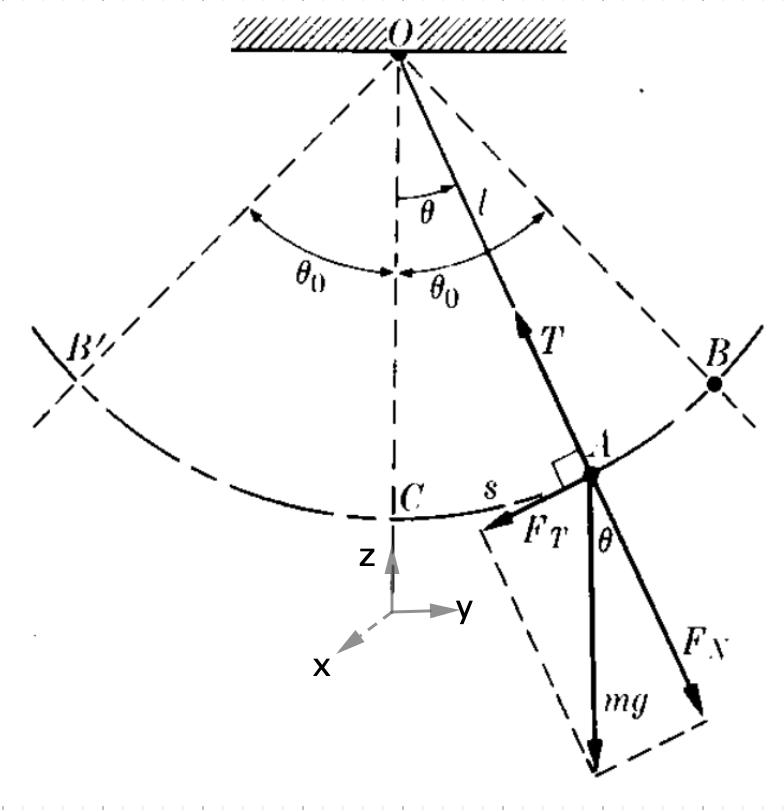
\includegraphics[width=.55\textwidth]{imagenes/imagenes19/T19IM06.png}
	\end{figure}
\end{multicols}

$\vec L=-ml^2 \displaystyle \dv{\theta}{t} \ \vec i$. Sustituyendo en la ecuación general del movimiento de rotación:

$\displaystyle \dv{t} \left( ml^2 \dv{\theta}{t} \ \vec i \right)=lmg\sin \theta \vec i \to -\cancel{m} l^{\cancel{2}}\dv[2]{\theta}{t}=\cancel{l}\cancel{m}g\sin \theta$

\begin{equation}
\displaystyle \boldsymbol{\dv[2]{\theta}{t} \ + \ \dfrac g l \ \sin \theta \ = \ 0} \qquad \text{Ec. gral. péndulo}
\end{equation}
 
Establecemos una condición restrictiva: consideraremos ángulos $\theta$ muy pequeños \textcolor{gris}{$(\theta<<1 \to \sin \theta \approx \theta)$}.

\begin{equation}
\displaystyle \boxed{\ \boldsymbol{\dv[2]{\theta}{t} \ + \ \dfrac g l \  \theta \ = \ 0}\ } \qquad \text{EDO péndulo simple.}
\end{equation}

Obtenemos la EDO \footnote{EDO: ecuación diferencial ordinario (segundo orden con coeficientes constantes) péndulo} del péndulo simple.

Comparando con los resultados anteriores, la solución de esta EDO es:

\begin{equation}
\boldsymbol{
\theta=\theta_0 \cos \left( \sqrt{\dfrac l g} \ t + \alpha \right)\ ; \qquad  \ T=2\pi \sqrt{\dfrac l g}
}	
\end{equation}

Para ángulos mayores que el considerado para la aproximación de ángulos pequeños, tenemos la expresión \textcolor{gris}{McLaurin}:

$$T=2\pi \sqrt{\dfrac l g} \ \left[ 1 + \dfrac 1 4 \sin^2 \dfrac {\theta}{2} + \dfrac 9{64} \sin^4 \dfrac{\theta}{2} + \cdots \right]$$

que, de nuevo para pequeños ángulos se queda en: 

$\ T=2\pi \sqrt{\dfrac l g} \left( 1+\dfrac{\theta}{16} \right) \qquad$
\textcolor{gris}{(errores $<1 \%$ para ángulos $<23^o$)}

\subsection{Péndulo físico o compuesto}
\begin{multicols}{2}
Cualquier cuerpo rígido suspendido por un hilo capaz de oscilar alrededor de un eje.$O$ centro de oscilación.

$\displaystyle \dv{\vec L}{t}=\vec M^{(e)}$, ecuación del movimiento se rotación.	

$\vec M^{(e)}=\vec b \times m\vec g=bmg\sin\theta \ \vec u_z$

$\vec L=I\vec \omega= -I \displaystyle \dv{\theta}{t} \ \vec u_z$ \textcolor{gris}{(por las mismas consideraciones de signos que en el péndulo simple.)}

$\displaystyle I \dv[2]{\theta}{t} + bmg\sin \theta=0$

$\boldsymbol{ \displaystyle \dv[2]{\theta}{t}+\dfrac{bmg}{I} \sin \theta =0 }$
\begin{figure}[H]
		\centering
		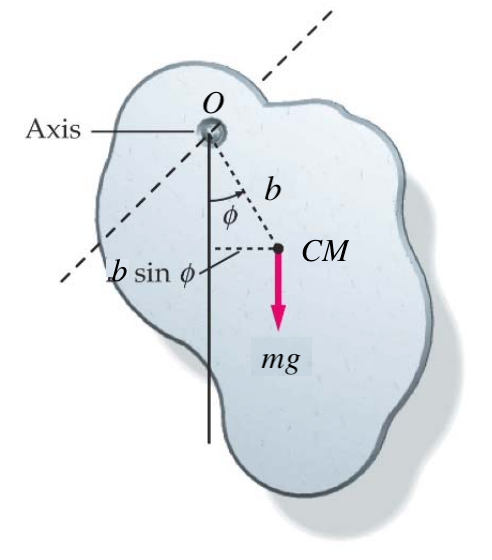
\includegraphics[width=.5\textwidth]{imagenes/imagenes19/T19IM07.png}
	\end{figure}	
\end{multicols}

$\theta << 1 \ \to \ \sin \theta \approx \theta \quad \Rightarrow \quad \boldsymbol{ \displaystyle \dv[2]{\theta}{t}+\dfrac{bmg}{I}  \theta =0 }$

$\omega=\dfrac{2\pi}{T}=\sqrt{\dfrac{bmg}{I}} \quad \to \quad \boldsymbol{ T=2\pi \sqrt{\dfrac{I}{bmg}}}$

Sustituyendo $I=mR^2$, con $R$ el radio de giro \textcolor{gris}{ ( $I=\int r^2 \dd m = m R^2$ ) }, es \textbf{como si} toma la masa estuviese concentrada en un punto a distancia $R$ tal que tuviese ese momento de inercia.

$ \boldsymbol{ T=2\pi \sqrt{ \dfrac{R^2}{bg} } }$. Si llamamos $l=\dfrac{R^2}{b}$ \emph{longitud equivalente del péndulo simple}, obtenemos el mismo resultado que el que teníamos para el péndulo simple.

Dos cuerpos que tengan la misma longitud equivalente oscilarán con el mismo periodo independientemente de la distribución de masa y de la masa que tengan.

 
\subsection{Péndulo de torsión}
\begin{multicols}{2}
Estando el sistema en régimen estacionario, por ``elasticidad'' sabemos que 

$M^{(e)}=-\dfrac{\pi \mu r^4}{2l}\theta=-k\theta$, 

$\mu$ coeficiente de cizalladura y $k$ coeficiente de torsión.

$L=i\omega=I\displaystyle \dv{\theta}{†}$

MAS $ \to \displaystyle \dv[2]{\theta}{t}+ \dfrac k I \theta = 0 \to \ T=2\pi \sqrt{\dfrac k I}$

El péndulo de torsión sirve para calcular el momento de inercia y el coeficiente de cizalladura. 
\begin{figure}[H]
		\centering
		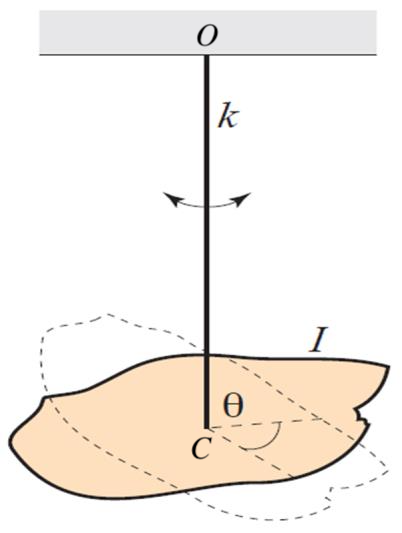
\includegraphics[width=.4\textwidth]{imagenes/imagenes19/T19IM08.png}
	\end{figure}	
\end{multicols}

\newpage %***********************************

\begin{myblock}{El oscilador armónico $\quad \boxed{\  \boldsymbol{\ddot x + \omega^2 x=0} \ }$}
El oscilador armónico es uno de los sistemas más estudiados en la física, ya que todo sistema que oscila al rededor de un punto de equilibrio estable se puede estudiar en primera aproximación como si fuera un oscilador.


\vspace{2mm} Se dice que un sistema cualquiera, mecánico,  eléctrico, neumático, etc., es un oscilador armónico si, cuando se deja en libertad fuera de su posición de equilibrio, vuelve hacia ella describiendo oscilaciones sinusoidales, o sinusoidales amortiguadas en torno a dicha posición estable.

\begin{figure}[H]
		\centering
		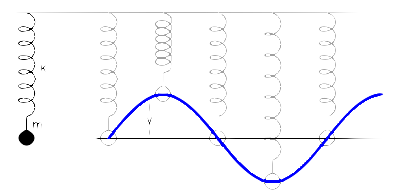
\includegraphics[width=1\textwidth]{imagenes/imagenes19/T19IM09.png}
	\end{figure}

\vspace{2mm} El ejemplo es el de una masa colgada a un resorte. Cuando se aleja la masa de su posición de reposo, el resorte ejerce sobre la masa una fuerza que es proporcional al desequilibrio (distancia a la posición de reposo) y que está dirigida hacia la posición de equilibrio. Si se suelta la masa, la fuerza del resorte acelera la masa hacia la posición de equilibrio. A medida que la masa se acerca a la posición de equilibrio y que aumenta su velocidad, la energía potencial elástica del resorte se transforma en energía cinética de la masa. Cuando la masa llega a su posición de equilibrio, la fuerza será cero, pero como la masa está en movimiento, continuará y pasará del otro lado. La fuerza se invierte y comienza a frenar la masa. La energía cinética de la masa va transformándose ahora en energía potencial del resorte hasta que la masa se para. Entonces este proceso vuelve a producirse en dirección opuesta completando una oscilación.

\vspace{2mm} Si toda la energía cinética se transformase en energía potencial y viceversa, la oscilación seguiría eternamente con la misma amplitud. En la realidad, siempre hay una parte de la energía que se transforma en otra forma, debido a la viscosidad del aire o porque el resorte no es perfectamente elástico. Así pues, la amplitud del movimiento disminuirá más o menos lentamente con el paso del tiempo. Se empezará tratando el caso ideal, en el cual no hay pérdidas. Se analizará el caso unidimensional de un único oscilador (para la situación con varios osciladores, véase movimiento armónico complejo).	
\end{myblock}

\vspace{5mm} %******************************************

